\chapter{Memory}

\begin{center}
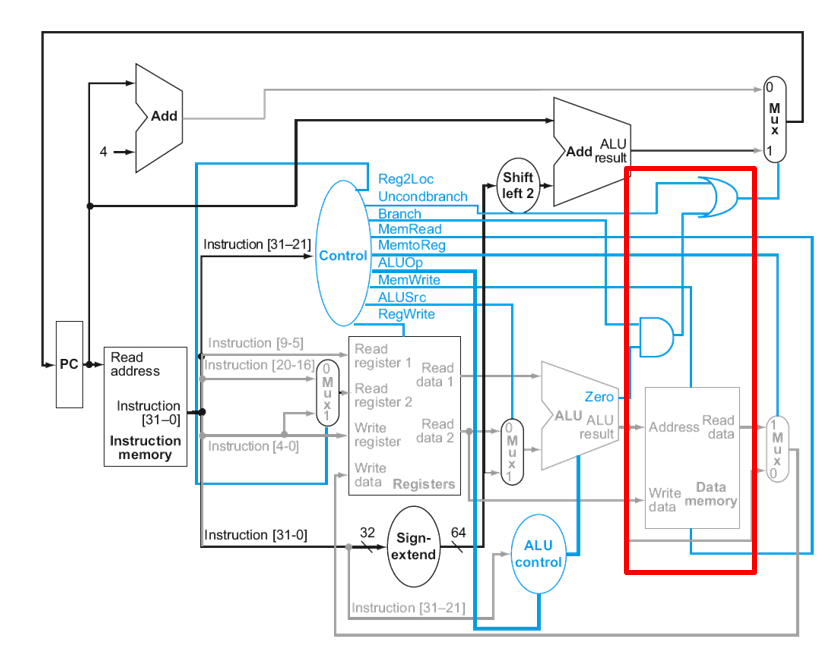
\includegraphics[width=5.5in]{../images/data_memory.png}
\end{center}

\section{Memory Stage}
Today we will create the iMemory stage of our processor.  This stage contains the data memory for the system that we use for load and store commands.  It also contains the logic gates used to produce the pc\_src signal that is used in the iFetch stage.  Note that although the diagram shows the pc\_src mux on the right side of the diagram, the mux is actually already implemented in the iFetch stage and belongs in the iFetch stage.

Because this module is so simple, we will put all of the code for the module in a new file called iMemory.v.  This file will read and write data memory as well as determine the branch result.

\section{Data Memory}

The data memory will be similar to the register file memory, with two primary changes:
\begin{enumerate}
	\item reading is now conditional on the MemRead control wire being high.  If the MemRead flag is not high, then the read\_data output should be set to Z (high impedance).
	\item writing is now permissible if the MemWrite control wire is high.
\end{enumerate}
In iMemory.v, copy the contents of register\_file.v and modify it to meet the needs of the data memory module.  I have provided a new data file, ramData.data that contains the initial values to be read into memory.

\section{Branch Resolution}

We now have all the information necessary to decide if the computer should branch or not.  We have the signal `branch' to tell us if it is a conditional branch command, and we have `zero' to tell us if the condition was met.  Both branch and zero must be true so we will combine them with an `and' gate.

We also need an 'or' gate to 'or' together the output of the 'and' gate (above) and the uncondBranch control signal.  These gates can be included directly in your iMemory module. While these are two separate gates on the Datapath Diagram, the code can be written as a single line of code (or you can write it as two lines, either way is fine).

\section{Test Bench}
For this lab, we will just have a single test bench that will test the entire iMemory stage.  The provided test bench is complete except that the cr values are not filled in.  Please fill in these values with the correct results that you expect to get.

\section{Your Assignment}

You are to:
\begin{enumerate}
\item Create a new module called iMemory as described above.
\item Update the testbench cr values to verify that the iMemory stage works properly. 
\item Rather than writing a lab report, please produce a landscape mode PDF file called Lab10\_lastname.pdf that includes (in this order):
\begin{enumerate}
	\item Your name and the lab number.
	\item A snip of the Simulation Results for the iMemory test.  Please show instructions in hex, opcodes and control signals in binary and everything else in signed decimal.  
	\item Copy and paste the entire log from BEGIN TEST RESULTS to END TEST RESULTS into your file.  The results have gotten too long to use the snipping tool.	
\end{enumerate}
\item Upload Lab10\_lastname.pdf file to Canvas.
\item Zip up your ARM-Lab directory and submit it on Canvas as well.  Please make sure that you give me the ARM-Lab directory rather than the ARM-Project directory.  I do not want the project files in the ARM-Project directory.  Before you submit your zip file, extract the file and make sure that the top-level directory is called ARM-Lab and that the lower level directories like code, manual, etc are directly beneath ARM-Lab in the directory structure.  I will extract your zip file and run your code against my correct testbench to verify that your code and testbench work correctly, and it is critical that everyone's directory structure is consistent.
\end{enumerate} 